\subsection{Obsługa grafiki za pomocą GDI}
\label{subsection_gdi}

\subsubsection{Podstawy GDI}

Podsystem GDI odpowiada za rysowanie elementów graficznych w specjalnie utworzonych
kontekstach urządzeń ({\em DC, Device Contexts}). 
Kontekst urządzenia może być skojarzony nie tylko z okiem, ale
także na przykład z wirtualnym obrazem strony tworzonej na drukarce. Dzięki takiemu podejściu
programista może użyć dokładnie tych samych mechanizmów do tworzenia obrazu na w oknie i na drukarce.

GDI jest jednym z najlepszych przykładów na to, że z perspektywy programisty nie tylko każda
odmiana systemu Windows zachowuje się tak samo, ale również każdy model PCta, choć przecież
zbudowany z innych podzespołów, identycznie reaguje na polecenia programisty. Nie ważne, czy
w komputerze mam najnowszy model karty graficznej, czy zwykłą kartę VGA, Windows na polecenie
narysowania linii na ekranie zareaguje tak samo.

Dzieje się tak dlatego, że między wywołaniem funkcji przez programistę, a pojawieniem się jej
efektów, system operacyjny wykonuje mnóstwo pracy, o której nawet programista nie ma pojęcia. W przypadku
GDI, Windows wysyła odpowiednie polecenia do {\bf sterownika ekranu}, który, co nie powinno dziwić, również
ma swój interfejs programowania, służący do porozumiewania się sterownika z systemem, tyle że ukryty
przed programistą pracującym z Win32API.

Zobaczmy przykład użycia GDI:

\begin{scriptsize}
\begin{verbatim}
/*
 *
 * Tworzenie grafiki za pomocą GDI
 *
 */
#include <windows.h>
#include <string.h>

/* Deklaracja wyprzedzająca: funkcja obsługi okna */
LRESULT CALLBACK WindowProcedure(HWND, UINT, WPARAM, LPARAM);
/* Nazwa klasy okna */
char szClassName[] = "PRZYKLAD";

int WINAPI WinMain(HINSTANCE hThisInstance, HINSTANCE hPrevInstance, 
                   LPSTR lpszArgument, int nFunsterStil)
{
    HWND hwnd;               /* Uchwyt okna */
    MSG messages;            /* Komunikaty okna */
    WNDCLASSEX wincl;        /* Struktura klasy okna */

    /* Klasa okna */
    wincl.hInstance     = hThisInstance;
    wincl.lpszClassName = szClassName;
    wincl.lpfnWndProc   = WindowProcedure;    // wskaźnik na funkcję obsługi okna  
    wincl.style         = CS_DBLCLKS;                 
    wincl.cbSize        = sizeof(WNDCLASSEX);

    /* Domyślna ikona i wskaźnik myszy */
    wincl.hIcon   = LoadIcon(NULL, IDI_APPLICATION);
    wincl.hIconSm = LoadIcon(NULL, IDI_APPLICATION);
    wincl.hCursor = LoadCursor(NULL, IDC_ARROW);
    wincl.lpszMenuName = NULL; 
    wincl.cbClsExtra = 0;   
    wincl.cbWndExtra = 0;   
    /* Jasnoszare tło */
    wincl.hbrBackground = (HBRUSH)GetStockObject(LTGRAY_BRUSH);

    /* Rejestruj klasę okna */
    if(!RegisterClassEx(&wincl)) return 0;

    /* Twórz okno */
    hwnd = CreateWindowEx(
           0,                   
           szClassName,         
           "PRZYKLAD",       
           WS_OVERLAPPEDWINDOW, 
           CW_USEDEFAULT,       
           CW_USEDEFAULT,       
           512,                 
           512,                 
           HWND_DESKTOP,        
           NULL,                
           hThisInstance,       
           NULL                 
           );

    ShowWindow(hwnd, nFunsterStil);
    /* Pętla obsługi komunikatów */
    while(GetMessage(&messages, NULL, 0, 0))
    {
           /* Tłumacz kody rozszerzone */
           TranslateMessage(&messages);
           /* Obsłuż komunikat */
           DispatchMessage(&messages);
    }

    /* Zwróć parametr podany w PostQuitMessage( ) */
    return messages.wParam;
}

int xSize, ySize;

/* Tę funkcję woła DispatchMessage( ) */
LRESULT CALLBACK WindowProcedure(HWND hwnd, UINT message, 
                                 WPARAM wParam, LPARAM lParam)
{
    char sText[] = "Przykład 1, witam";
    HDC         hdc ; // kontekst urządzenia
    int         i ;
    PAINTSTRUCT ps ;
    RECT r;

    HPEN   hPen;
    HBRUSH hBrush;
    
    switch (message)                  
    {
           case WM_DESTROY:
              PostQuitMessage(0);        
              break;
           case WM_SIZE:
              xSize = LOWORD(lParam); 
              ySize = HIWORD(lParam); 
              
              GetClientRect( hwnd, &r );
              InvalidateRect( hwnd, &r, 1 );
              
              break;   
           case WM_PAINT:
              hdc = BeginPaint (hwnd, &ps) ;
                      
              // linie             
              hPen = CreatePen (PS_SOLID, 3, RGB (255, 0, 0)) ;
              SelectObject( hdc, hPen );              
              for ( i=0; i<xSize; i+=xSize/40 )               
              {
                 MoveToEx( hdc, xSize/2, 0, NULL );
                 LineTo( hdc, i, ySize );
              }   
              DeleteObject( hPen );
          
              // kształty
              SetBkColor( hdc, RGB(0, 255, 0) );
              hBrush = CreateHatchBrush (HS_CROSS, RGB (0, 0, 255)) ;
              SelectObject( hdc, hBrush );
              r.left   = 10;
              r.top    = 10;
              r.right  = 50;
              r.bottom = 50;
              FillRect( hdc, &r, hBrush );              
              DeleteObject( hBrush );

              // tekst
              if ( xSize > 0 && ySize > 0 )
              {
                 SetTextAlign( hdc, TA_CENTER | VTA_CENTER );
                 SetBkMode( hdc, TRANSPARENT );
                 TextOut( hdc, xSize / 2, 20, sText, strlen( sText ) );
              }
          
              EndPaint(hwnd, &ps);
              break;   
              
           default:                   
              return DefWindowProc(hwnd, message, wParam, lParam);
    }
    return 0;
}
\end{verbatim}
\end{scriptsize}

Jak widać obiektów GDI używa się w sposób dość prosty. Obiekt jest najpierw tworzony
za pomocą odpowiedniej funkcji (na przykład {\bf CreatePen}), następnie jest ustawiany jako
bieżący (za pomocą funkcji {\bf SelectObject}), zaś po użyciu jest niszczony ({\bf DeleteObject}).

\begin{figure}
\begin{center}
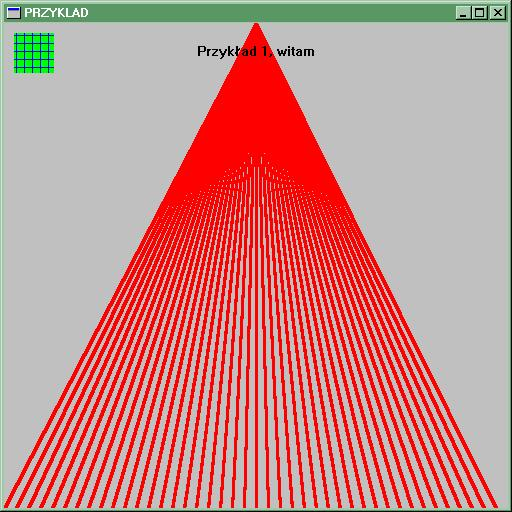
\includegraphics[width=0.5\textwidth]{./pic/p03}
\caption{Obsługa grafiki okna za pomocą GDI}
\end{center}
\end{figure}

\subsubsection{Uchwyty do kontekstów urządzeń}

Wszystkie funkcje GDI, które odpowiadają za tworzenie obrazu, przyjmują jako pierwszy 
parametr uchwyt do kontekstu urządzenia. Dzięki temu system wie do jakiego obiektu (okna, drukarki)
odnosi się aktualna funkcja. 

W przypadku rysowania w oknach, kontekst urządzenia można uzyskać na dwa sposoby.

\begin{description}
\item[Wewnątrz WM\_PAINT] W kodzie obsługującym komunikat WM\_PAINT uchwyt kontekstu 
	można pobrać i zwolnić za pomocą funkcji
\begin{scriptsize}
\begin{verbatim}
HDC BeginPaint(

    HWND hwnd,	
    LPPAINTSTRUCT lpPaint	
   );	

BOOL EndPaint(

    HWND hWnd,	
    CONST PAINTSTRUCT *lpPaint 	
   );
\end{verbatim}
\end{scriptsize}

\item[Poza WM\_PAINT] Poza kodem obsługującym komunikat WM\_PAINT uchwyt kontekstu 
	można pobrać i zwolnić za pomocą funkcji
\begin{scriptsize}
\begin{verbatim}
HDC GetDC(

    HWND hWnd 	
   );	

HDC GetWindowDC(

    HWND hWnd 	
   );

int ReleaseDC(

    HWND hWnd,	
    HDC hDC 	
   );	
\end{verbatim}
\end{scriptsize}

\end{description}

Skąd system Windows wie, kiedy do okna przesłać komunikat WM\_PAINT oznaczający konieczność
odświeżenia zawartości okna? Otóż z każdym oknem system kojarzy informację o tym, czy jego
zawartość jest ważna, czy nie. 

Po zakończeniu rysowania i wywołaniu funkcji {\bf EndPaint}, zawartość
okna jest ważna. Kiedy okno zostanie na przykład przykryte innym oknem, a następnie odsłonięte z powrotem
lub na przykład zminimalizowane a następnie przywołane z powrotem, Windows automatycznie wysyła do okna komunikat
WM\_PAINT, uznając powierzchnię okna za nieważną.

Bardzo często okazuje się, że programista chce powierzchnię okna unieważniać częściej niż gdyby miało dziać się
to automatycznie. Na przykład wtedy, kiedy zawartość okna musi być odświeżana regularnie, ponieważ zawiera
jakieś chwilowe, ulotne informacje. W takim przypadku obszar okna może być unieważniany 
bądź zatwierdzany za pomocą funkcji:

\begin{scriptsize}
\begin{verbatim}
BOOL InvalidateRect(

    HWND hWnd,	
    CONST RECT *lpRect,	
    BOOL bErase	
   );

BOOL ValidateRect(

    HWND hWnd,	
    CONST RECT *lpRect	
   );
\end{verbatim}
\end{scriptsize}

Pierwsza z tych funkcji powoduje natychmiastowe wysłanie do okna komunikatu WM\_PAINT, druga zaś powoduje
zatwierdzenie obszaru okna. System traktuje komunikat WM\_PAINT w sposób trochę szczególny, bowiem wysyłanie
tego komunikatu cześciej niż jest on obsługiwany nie ma żadnego efektu - w kolejce komunikatów do 
okna może znajdować się w danej chwili tylko jeden komunikat WM\_PAINT.

\subsubsection{Własne kroje pisma}

Własne kroje pisma można tworzyć za pomocą funkcji
\begin{scriptsize}
\begin{verbatim}
HFONT CreateFont(

    int nHeight,	
    int nWidth,	
    int nEscapement,	
    int nOrientation,	
    int fnWeight,	
    DWORD fdwItalic,	
    DWORD fdwUnderline,	
    DWORD fdwStrikeOut,	
    DWORD fdwCharSet,	
    DWORD fdwOutputPrecision,	
    DWORD fdwClipPrecision,	
    DWORD fdwQuality,	
    DWORD fdwPitchAndFamily,	
    LPCTSTR lpszFace 	
   );
\end{verbatim}
\end{scriptsize}

Aby utworzona czcionka stała się aktywna należy oczywiście wybrać ją w jakimś kontekście graficznym za pomocą
funkcji {\bf SelectObject}.